\documentclass[fleqn]{exam}
\usepackage[utf8]{inputenc}
\usepackage{mathtools, gensymb}
\usepackage{tikz}
\usepackage{tkz-euclide}
\usepackage[siunitx]{circuitikz}
\usepackage{amsmath}
\usepackage{cancel}
\usepackage{pgfplots}
\usepackage{graphicx}

\title{Verifica Telecomunicazioni}
\author{Saronni Gabriele}
\date{06 Giugno 2020}

\begin{document}
\begin{titlepage}
\maketitle
\end{titlepage}
\section{Verifica di geometria e piano cartesiano}
\begin{enumerate}
    \item Se il cateto orizzontale $c_2$ è 24 e l'ipotenusa $i$ è 25: \\
    Determinare l'angolo $\beta$, l'angolo $\gamma$ ed il cateto $c_1$ rappresentati in figura. \\
    
    \begin{center}
        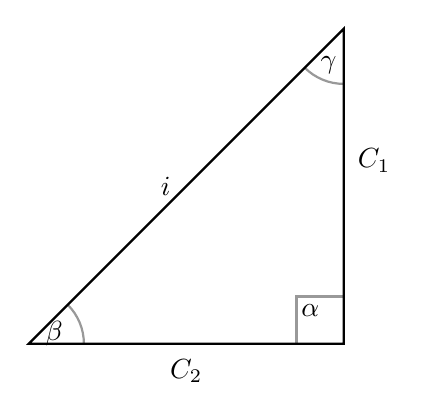
\begin{tikzpicture}[thick]
            \coordinate (O) at (0,0);
            \coordinate (A) at (4,0);
            \coordinate (B) at (4,4);
            \draw (O)--(A)--(B)--cycle;
            
            \tkzLabelSegment[below=2pt](O,A){\textit{$C_2$}}
            \tkzLabelSegment[left=2pt](O,B){\textit{$i$}}
            \tkzLabelSegment[above right=2pt](A,B){\textit{$C_1$}}
            
            \tkzMarkAngle[size=0.7,opacity=.4](A,O,B)
            \tkzLabelAngle[pos = 0.35](A,O,B){$\beta$}
            
            \tkzMarkRightAngle[size=0.6,opacity=.4](B,A,O) % square angle here
            \tkzLabelAngle[pos = 0.6](B,A,O){$\alpha$}
            
            \tkzMarkAngle[size=0.7cm,opacity=.4](O,B,A)
            \tkzLabelAngle[pos = 0.5](O,B,A){$\gamma$}
        \end{tikzpicture}
    \end{center}
	
    $C_2 = 24$ \\
    $i = 25$ \\
    $\beta = ?$ \\
    $\gamma = ?$ \\
    $C_1 = ?$

    Avendo $C_2$ e $i$ possiamo ottenere $C_1$ = $\sqrt{i^2-C_2^2}$ \\
    $C_1 = \sqrt{25^2-24^2} = 7$ \\
    \\ 
    Per ottenere gli angoli rimanenti possiamo usare: $\alpha = \tan^{-1}\Big(\frac{i}{C_2}\Big)$ \\
    \\ 
    $\beta = \tan^{-1}\Big(\frac{C_1}{C_2}\Big) = \tan^{-1}\Big(\frac{7}{24}\Big) = 16.26\degree$\\
    $\gamma = \tan^{-1}\Big(\frac{C_2}{C_1}\Big) = \tan^{-1}\Big(\frac{24}{7}\Big) = 73.74\degree$ 
    
    \item In relazione all'esercizio precedente, se il cateto orizzontale $C_2$ si dimezza: \\
    Determinare l'angolo $beta$, l'angolo $\gamma$ e l'ipotenusa $i$ ($C_1$ rimane uguale).
    
	$C_1 = 7$ \\
    $C_2 = 12$ \\
    $\beta = ?$ \\
    $\gamma = ?$ \\
    $i = ?$ 


    Avendo $C_1$ e $C_2$ possiamo ottenere $i = \sqrt{C_1^2+C_2^2}$ \\
    $i = \sqrt{7^2+12^2} = 13.89$ \\
    \\ 
    Per ottenere gli angoli rimanenti possiamo usare: $\alpha = \tan^{-1}\Big(\frac{i}{C_2}\Big)$ \\
    \\ 
    $\beta = \tan^{-1}\Big(\frac{C_1}{C_2}\Big) = \tan^{-1}\Big(\frac{7}{12}\Big) = 30.25\degree$\\
    $\gamma = \tan^{-1}\Big(\frac{C_2}{C_1}\Big) = \tan^{-1}\Big(\frac{12}{7}\Big) = 59.74\degree$ 
    
\pagebreak    
    
    \item Determina e rappresenta nel grafico l'angolo ed il modulo dei seguenti punti. \\
    A ($-5, -2$) \\
    B ($-3, 1$) \\
    C ($7, -4$) \\
    \\
    Modulo = $\sqrt{x^2+y^2}$ \\
	Angolo = $\tan^{-1}\Big(\frac{y}{x}\Big)$ \\

    A: \\
    Modulo = $\sqrt{(-5^2)+(-2^2)} = 5.38$ \\
	Angolo = $\tan^{-1}\Big(\frac{-2}{-5}\Big) = 21.80\degree$ \\
    
    B: \\
    Modulo = $\sqrt{(-3^2)+(1^2)} = 3.16$ \\
	Angolo = $\tan^{-1}\Big(\frac{1}{-3}\Big) = -18.43\degree$ \\
    
    C: \\
    Modulo = $\sqrt{(7^2)+(-4^2)} = 8.06$ \\
	Angolo = $\tan^{-1}\Big(\frac{-4}{7}\Big) = -29.74\degree$ \\
    
    %axis lines=middle,axis equal,grid=both
    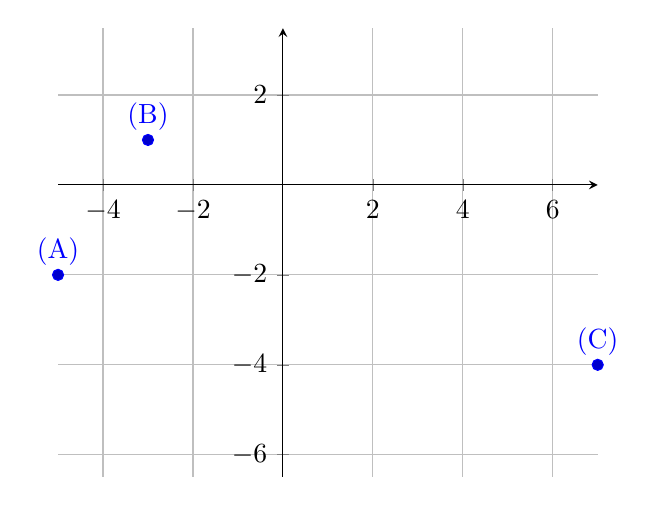
\begin{tikzpicture}
	\begin{axis}[nodes near coords,enlargelimits=0.2,axis lines=middle,axis equal,grid=both]
    \addplot+ [only marks,
    point meta=explicit symbolic,] coordinates {
        (-5,-2) [(A)]
        (-3,1) [(B)]
        (7,-4) [(C)]
        };
	\end{axis}
	\end{tikzpicture}
    
    
\end{enumerate}

\pagebreak

\section{Verifica di teoria circuitale di base}
In relazione al circuito sottostante dove $V = 270V$, $R_1 = 1\Omega$, $R_2 = 3\Omega$ e $R_3 = 6\Omega$ determinare: \\
\textbf{NOTA:} \emph{Disegnare il verso della corrente uscente dal generatore presa con la convenzione del generatore e le cadute di tensione sulle resistenze con la convenzione dell'utilizzatore.}
\\
\begin{center}

    \begin{circuitikz} \draw (0,0)
        to[V,v=V, *-*] (0,6) % The voltage source
        (0,6) -- (2,6)
        to [R, l=$R_1$, *-](2, 4) % The resistor
        to [R, l=$R_2$](2, 2) % The resistor
        to [R, l=$R_3$, -*](2, 0) % The resistor
        (2,0) -- (0,0);
    \end{circuitikz}

\end{center}
	
    \begin{itemize}
        \item La corrente $I$ e le cadute di tensione $v_1$, $v_2$ e $v_3$. Con la verifica del risultato tramite la legge di Kirchoff alla maglia.
        
        \begin{align*}
        	&V = 270V \\
            &R_1 = 1\Omega \\
            &R_2 = 3\Omega \\
            &R_3 = 6\Omega \\ \\
            &I = ? \\
            &v_1 = ? \\
            &v_2 = ? \\
            &v_3 = ? \\ \\
            &R = \frac{V}{I} \\
            &V = I \cdot R \\
            &I = \frac{V}{R} \\ \\
            &I = \frac{270}{1} = 270 A \\
            &I = \frac{270}{3} = 90 A \\
            &I = \frac{270}{6} = 45 A \\
            &
        \end{align*}
        
        \item Le cadute di tensione $v_1$, $v_2$ e $v_3$ tramite il partitore di tensione e determinare i potenziali elettrici ai nodi di ogni resistenza.
    \end{itemize}

    \begin{align*}
        &V = 270V \\
        &R_1 = 1\Omega \\
        &R_2 = 3\Omega \\
        &R_3 = 6\Omega \\ \\
        &v_1 = ? \\
        &v_2 = ? \\
        &v_3 = ? \\
    \end{align*}

\pagebreak

\section{Verifica doppi bipoli}
    \begin{enumerate}
        \item Determinare il guadagno di un amplificatore, con potenza in ingresso di $30 mW$, che fornisce in uscita $3,5 W$.
        \item Un segnale da $45 mW$ subisce un'attenuazione di $12 dB$. Determinare la potenza del segnale al termine in $mW$ ed in $dBm$.
        \item Un segnale da $2 mW$ viene amplificato con un guadagno di $10 dB$. Determinare la potenza del segnale al termine in $mW$ ed in $dBm$.
    \end{enumerate}

\pagebreak

\section{Verifica Serie di Fourier}
    \begin{enumerate}
        \item Compilare le tabelle relative ai seguenti segnali di corrente e plottarne lo spettro
    
    	\begin{center}
        \includegraphics{fourier.png}        
        \end{center}

        \item Segnale ad onda quadta di picco $A = 2,3 uA$ e frequenza $f = 560kHz$
        \item Segnale a onda triangolare di picco $A = 19,3 mA$ e frequenza $f = 2,5MHz$
        \begin{center}
        \includegraphics{tableaa.png}\\
        \includegraphics{tableB.png}\\
        \end{center}
    \end{enumerate}
\end{document}
